%/Users/jinboyu/Downloads/Written Report (1)%!TEX encoding=UTF-8
%!TEX program=xelatex
\documentclass[pre,twocolumn,floatfix]{revtex4-1}
\usepackage{xeCJK} %使用xeCJK宏包
\usepackage{graphicx} % Include figure files
\usepackage{braket}   
\usepackage{tikz}   
\usepackage{booktabs}
\usepackage{tabularx}
\usepackage{array}
\usepackage{subcaption}
\usepackage{amsfonts}
\usepackage{amssymb}
\usepackage[export]{adjustbox}
\usepackage{listings}
\usepackage{xcolor}
\usepackage{float}
\lstset{
    basicstyle=\ttfamily\footnotesize,
    breaklines=true,
    frame=single,
    columns=fullflexible,
    keepspaces=true,
    language=Python
} 
\graphicspath{ {images/} }
\usetikzlibrary{quantikz}

\begin{document}

\title{《量子信息基础》课题报告}

\author{金泊宇}
\affiliation{浙江大学竺可桢学院,杭州 310058}

\author{刘昕昀}
\affiliation{浙江大学竺可桢学院,杭州 310058}


\date{\today}

\begin{abstract}
This report investigates the application of Quantum Neural Networks (QNNs) to find the ground states of the one-dimensional transverse-field quantum Ising model, enabling a deeper investigation into quantum phase transitions. The results obtained from the QNN approach are then compared with the exact diagonalization method, which provides the true ground-state energy, transverse magnetization, and longitudinal magnetization. We explore the accuracy and efficiency of QNNs for simulating quantum many-body systems and discuss the potential advantages and limitations of this variational approach.
\end{abstract}

\maketitle


\section{Introduction} \label{1}%------------------------------
The quantum Ising model is a fundamental model in condensed matter physics, describing a system of interacting spins subjected to a transverse magnetic field. It plays a crucial role as a testbed for both theoretical analysis and computational techniques because of its exact solvability in one dimension and its relevance to quantum phase transitions. Although exact diagonalization offers highly accurate results for small system sizes, its computational cost grows exponentially with the number of spins, rendering it impractical for larger systems. This limitation motivates the exploration of alternative classical methods, as well as the potential application of Quantum Neural Networks (QNNs) to efficiently approximate ground states and gain further insight into quantum critical phenomena.



\section{The Transverse Field Quantum Ising Model}

The transverse field quantum Ising model (TFQIM) is a prototypical model in quantum many-body physics. It describes a one-dimensional chain of spin-$\frac{1}{2}$ particles with nearest-neighbor interactions along the $z$-axis and a uniform transverse magnetic field applied in the $x$-direction. This model is particularly significant, as it exhibits a quantum phase transition - a fundamental change in the ground state of the system driven by quantum fluctuations - when the ratio of the transverse field $h$ to the coupling strength $J$ is varied.

The Hamiltonian for the one-dimensional transverse field quantum Ising model is given by:
\begin{equation}
    H = -J \sum_{i=1}^{N} \sigma_i^{z} \sigma_{i+1}^{z} - h \sum_{i=1}^{N} \sigma_i^{x}
\end{equation}
where:
\begin{itemize}
    \item $N$ is the number of spins in the chain.
    \item $J$ is the strength of the nearest-neighbor spin coupling (we set $J = 1$ for simplicity).
    \item $h$ is the strength of the transverse magnetic field.
    \item $\sigma_i^z$ and $\sigma_i^x$ are Pauli matrices acting on the $i$-th spin.
    \item Periodic boundary conditions are often assumed, that is, $\sigma^z_{N+1} = \sigma^z_1$.
\end{itemize}

The ground-state energy of this Hamiltonian corresponds to its lowest eigenvalue. 


%----------------------------------2------------------------------------------


\section{Quantum Phase Transitions} \label{sec:quantum-phase-transitions}%------------------------------
\subsection{Introduction}
 A quantum phase transition refers to a qualitative change in the ground state of a quantum system as a function of some external parameter, typically the interaction strength, magnetic field, or pressure, at zero temperature. Unlike classical phase transitions that are driven by thermal fluctuations, quantum phase transitions arise from quantum fluctuations and occur at absolute zero, where thermal energy is absent.

Formally, a quantum phase transition is signaled by a nonanalyticity in the ground-state energy of the Hamiltonian $H(g)$ as a function of a control parameter $g$. These nonanalytic behaviors are generally associated with avoided level crossings in finite-size systems, which become true level crossings in the thermodynamic limit ($N \to \infty$). Figure~\ref{1} illustrates such a scenario where energy levels come close together in a finite system, indicating a possible quantum phase transition in the large-$N$ limit.

\begin{figure}
    \centering
    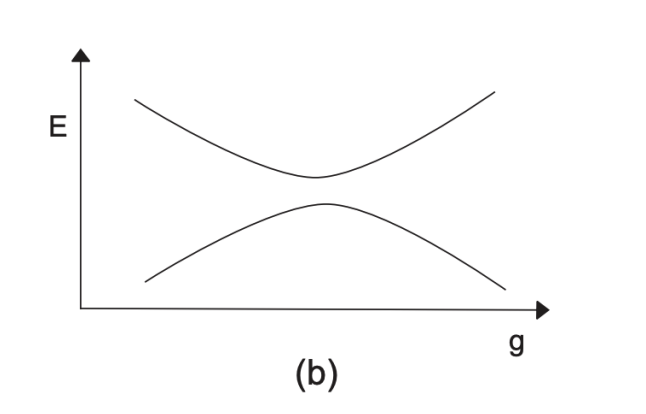
\includegraphics[width=0.5\linewidth]{images/截屏2025-05-22 21.25.44.png}
    \caption{Shown above is a near level crossing for finite system that can become non-analytic in the infinite system limit. }
    \label{fig:level-crossing}
\end{figure}

 \subsection{Phase Transition in the Transverse-Field Ising Model}
We can provide heuristic arguments for the existence of a quantum phase transition in the 1D transverse-field Ising
model of Equation 1. For $g\ll1$, the nearest-neighbour coupling term dominates and the ground state is expected
to be such that all spins are completely aligned in the up or down direction. For $g\gg1$, the external field dominates
and the ground state is expected to have all spins aligned with the external field.

In the $g\ll1$ case, there is a $\mathbb{Z}_2$ symmetry in the ground state corresponding to the flipping of the spins along the z-axis $\sigma_i^z\to-\sigma_i^z$. The spontaneous $\mathbb{Z}_2$ symmetry break as $g\to0$ is indicative of a phase transition at some critical
coupling $g_c$ of order one. The transverse-field Ising model, parameterized as in Equation 1 has this quantum phase
transition described above at $T=0\implies J\to\infty$, where the ground state level crossing is most important.





% -----------------------------------3----------------------------------------
\section{Classical Solutions}
To investigate the ground state properties of the transverse-field Ising model—such as the ground state energy and magnetization in the x- and z-directions—various classical computational techniques have been developed, including exact diagonalization (ED), density matrix renormalization group (DMRG), and Jordan-Wigner transformation-based approaches. In this section, we introduce ED and DMRG, which will later be used to evaluate the accuracy of the Quantum Neural Network (QNN) results. 
\subsection{Exact Diagonalization (ED)}
Exact diagonalization (ED) is a straight-forward numerical technique used to solve quantum many-body systems by directly computing the eigenvalues and eigenvectors of the system's Hamiltonian matrix. It is one of the most accurate methods available, as it provides exact solutions for quantities such as the ground state energy, wavefunction, and expectation values of observables.

In ED, the full Hamiltonian is represented as a $2^N \times 2^N$ matrix, where $N$ is the number of qubits. The exponential growth of the Hilbert space with system size limits this method to small systems---typically $N \lesssim 20$---depending on available computational resources.

Because of its exactness and transparency, ED is widely used to study quantum phase transitions. In our work, due to the size limitation of QNN method, ED serves as the main approach to evaluate the accuracy of QNN.


\subsection{Density Matrix Renormalization Group (DMRG)}
The Density Matrix Renormalization Group (DMRG) is a powerful numerical method for studying the ground state properties of low-dimensional quantum many-body systems, particularly in one dimension. Introduced by S.~R.~White in the early 1990s, DMRG has become one of the most accurate techniques for solving strongly correlated models such as the transverse-field Ising model. It is especially well-suited for computing the ground state energy and local observables (e.g., magnetization) of large systems, where exact diagonalization becomes intractable.

\subsubsection{Basic Procedure.}
DMRG works by iteratively constructing a large quantum system from smaller blocks while optimally truncating the Hilbert space to retain only the most relevant quantum states. The typical DMRG setup considers a one-dimensional chain divided into four parts: a system block (S), an environment block (E), and two physical sites between them. At each step, a "superblock" Hamiltonian is built from these components, and its ground state is calculated.

The key steps of the DMRG algorithm are:
\begin{enumerate}
    \item Initialize a small system block and environment block, each typically starting with one or two physical sites.
    \item Grow the system by adding one site to both the system and environment blocks to form a superblock.
    \item Diagonalize the superblock Hamiltonian to obtain its ground state.
    \item Compute the reduced density matrix of the system block by tracing out the environment.
    \item Retain only the $m$ eigenstates of the reduced density matrix with the largest eigenvalues to truncate the Hilbert space optimally.
    \item Use these truncated basis states to form the new system block and repeat the process.
\end{enumerate}

\begin{figure}
    \centering
    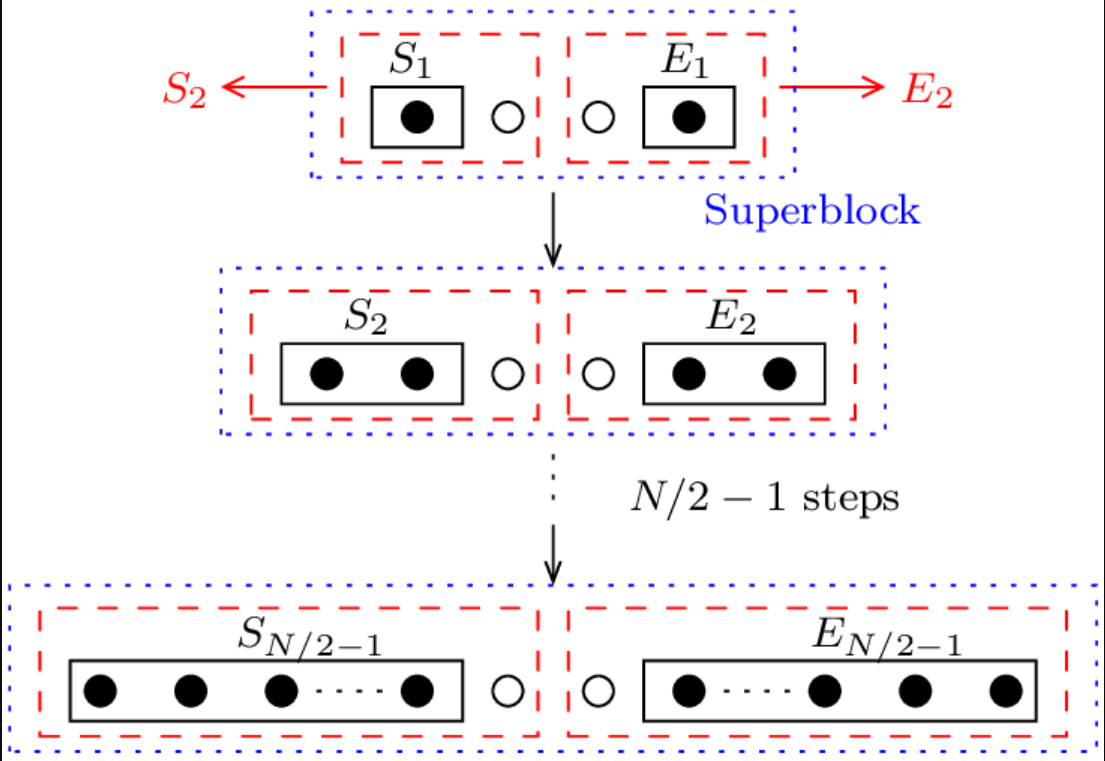
\includegraphics[width=0.5\linewidth]{屏幕截图 2025-05-30 165036.png}
    \caption{Shown above is the illustration of the basic procedure of DMRG}
    \label{fig:enter-label}
\end{figure}

After sweeping through the entire chain from left to right, a reverse sweep is performed (right to left) to refine the environment blocks using the now well-optimized system blocks. This two-way sweeping continues until convergence is achieved.

\subsubsection{Advantages.}
One of the key strengths of DMRG lies in its ability to drastically reduce the effective Hilbert space dimension by retaining only the most significant quantum states. While exact diagonalization requires handling the full Hilbert space of dimension $2^N$ for a system of $N$ spin-$\tfrac{1}{2}$ particles, DMRG keeps only the top $m$ eigenstates of the reduced density matrix. This allows each superblock to operate in a Hilbert space of dimension $m^2 \cdot d^2$, where $d$ is the local dimension (typically $d=2$), as opposed to the full $2^N$ scaling.

This efficient truncation ensures that DMRG scales polynomially with system size and remains tractable for large $N$. In addition, DMRG is variational, so the obtained ground state energy is an upper bound to the true ground state energy. It also provides accurate access to local observables such as magnetization in the $x$- and $z$-directions. These features make DMRG an ideal benchmark for evaluating the performance of variational quantum algorithms when N becomes large.

% -----------------------------------4----------------------------------------
\section{Quantum Machine Learning Method} 
\subsection{Introduction}
Quantum Machine Learning represents the intersection of quantum computing and classical machine learning techniques, offering potential advantages in:
\begin{itemize}
    \item Computational speedups for certain problems.
    \item Enhanced model expressivity through quantum feature maps.
    \item Novel learning paradigms leveraging quantum effects.
\end{itemize}

QML algorithms typically fall into two main categories:
\begin{enumerate}
    \item Quantum-enhanced classical ML (processing classical data).
    \item Quantum-native ML (processing quantum data).
\end{enumerate}
Within this framework, \textbf{Variational Quantum Algorithms (VQAs)} and \textbf{Quantum Neural Networks (QNNs)} have emerged as particularly promising approaches for the NISQ (Noisy Intermediate-Scale Quantum) era.

\subsection{Key Branches}
\subsubsection{Variational Quantum Algorithms (VQAs)}
VQAs are hybrid quantum-classical algorithms that use:
\begin{enumerate}
    \item A \textbf{parameterized quantum circuit (ansatz)} to prepare trial states.
    \item \textbf{Quantum hardware} to evaluate cost functions.
    \item \textbf{Classical optimizers} to adjust parameters.
\end{enumerate}

Key characteristics:
\begin{itemize}
    \item Suitable for noisy intermediate-scale quantum (NISQ) devices.
    \item Framework includes VQE (Variational Quantum Eigensolver), QAOA, and others.
    \item Requires careful ansatz design and parameter optimization.
\end{itemize}

\begin{figure}[H]
    \centering
    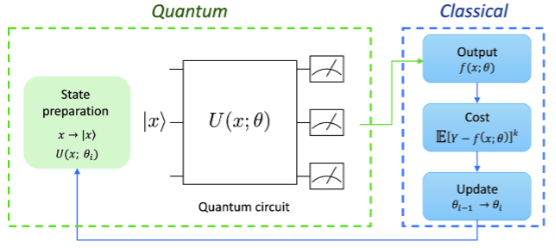
\includegraphics[width=0.5\linewidth]{images/qml.png}
    \caption{VQAs}
    \label{2}
\end{figure}

\subsubsection{Quantum Neural Networks (QNNs)}
QNNs extend classical neural networks by:
\begin{enumerate}
    \item Using quantum circuits as computational units.
    \item Encoding data in quantum states.
    \item Employing quantum measurements as nonlinear activations.
\end{enumerate}

\begin{figure}[H]
    \centering
    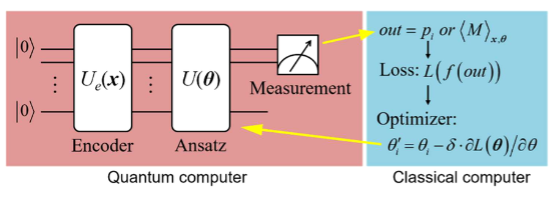
\includegraphics[width=0.5\linewidth]{images/QNN.png}
    \caption{QNNs}
    \label{3}
\end{figure}

In this implementation:
\begin{itemize}
    \item We used Qiskit's \verb|EstimatorQNN| as the quantum neural network.
    \item The \textbf{TorchConnector} enabled integration with PyTorch's optimization framework.
    \item The network was trained to minimize the energy expectation value.
\end{itemize}

\subsection{Methodology}
\subsubsection{Construct the Hamiltonian}
Use Qiskit's \verb|SparsePauliOp| to represent each Pauli term, which is concise and efficient.
    \begin{equation}
         H=-J\sum_i^N\sigma_i^{z}\sigma_{i+1}^{z}-h\sum_i^N\sigma_i^x
    \end{equation}
In which we can easily put $J=1$, and change the $h$ to represent the magnitude of the field strength over coupling.

\textbf{Pseudocode:}
\begin{lstlisting}[language=Python]
   FUNCTION build_ising_hamiltonian(n, J, h):
    // Initialize empty lists to store Pauli strings and their coefficients
    SET paulis = empty list
    SET coeffs = empty list

    // --- Construct Z_i Z_{i+1} terms (interaction terms) ---
    // Loop through each pair of adjacent qubits (from 0 to n-2)
    FOR i FROM 0 TO n - 2:
        // Create a list of 'I' (Identity) operators for all n qubits
        SET label = list of 'I' repeated n times

        // Set the i-th qubit's operator to 'Z'
        SET label[i] = 'Z'

        // Set the (i+1)-th qubit's operator to 'Z'
        SET label[i + 1] = 'Z'

        // Join the list into a string and reverse it (Qiskit's convention)
        ADD JOIN(REVERSE(label)) to paulis list

        // Add the coefficient -J for this term
        ADD -J to coeffs list
    END FOR

    // --- Construct X_i terms (transverse field terms) ---
    // Loop through each individual qubit (from 0 to n-1)
    FOR i FROM 0 TO n - 1:
        // Create a list of 'I' (Identity) operators for all n qubits
        SET label = list of 'I' repeated n times

        // Set the i-th qubit's operator to 'X'
        SET label[i] = 'X'

        // Join the list into a string and reverse it (Qiskit's convention)
        ADD JOIN(REVERSE(label)) to paulis list

        // Add the coefficient -h for this term
        ADD -h to coeffs list
    END FOR

    // Combine the Pauli strings and coefficients into a SparsePauliOp object
    // by zipping them together into a list of (Pauli_string, coefficient) tuples
    RETURN SparsePauliOp.from_list(ZIP(paulis, coeffs))

END FUNCTION

\end{lstlisting}[language=Python]
\subsubsection{physically inspired ansatz}
Design a variational circuit with:
\begin{itemize}
    \item \textbf{Initial state preparation:} RY gates with $\theta = 2arctan(h/J)$.
    \item \textbf{Layered structure:}
    \begin{enumerate}
        \item Alternating single-qubit RY and RX rotations.
        \item Nearest-neighbor CNOT entangling gates.
        \item Multi-repetitions (we put 4 in the training) of the ansatz layers.
    \end{enumerate}
\end{itemize}

\begin{figure}[htbp]
    \centering
    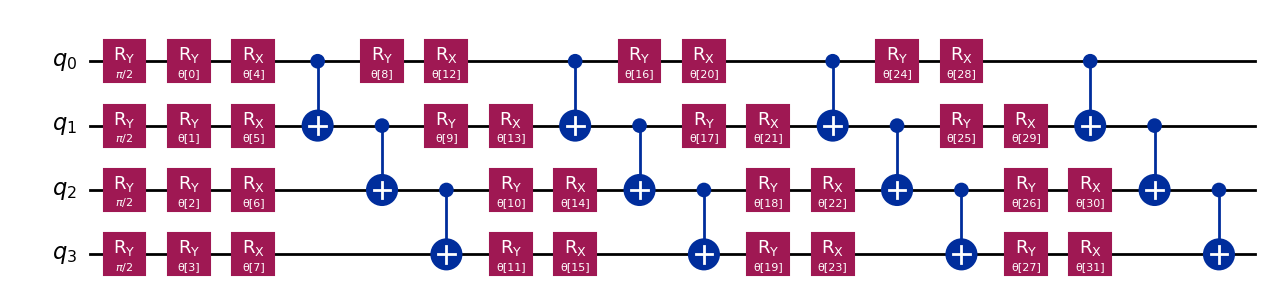
\includegraphics[width=0.5\linewidth]{images/ansatz.png}
    \caption{Ansatz circuit (qubits=4 and repetitions=4)}
    \label{4}
\end{figure}

\textbf{Pseudocode:}
\begin{lstlisting}[language=Python]
    FUNCTION create_physically_inspired_ansatz(n_qubits, h, J, reps = 3):
    // Initialize a vector of symbolic parameters
    SET params = new ParameterVector with name '\theta' and length (2 * n_qubits * reps)

    // Initialize a quantum circuit with n_qubits
    SET qc = new QuantumCircuit with n_qubits

    // --- Initial State Preparation ---
    // Calculate an initial rotation angle based on h and J
    SET init_angle = 2 * ARCTAN(h / J)

    // Apply RY rotation to each qubit for initial state preparation
    FOR i FROM 0 TO n_qubits - 1:
        APPLY RY_gate(init_angle) to qubit i
    END FOR

    // --- Ansatz Part: Multi-layer Rotation and Entanglement ---
    // Loop for the specified number of repetitions (layers)
    FOR rep FROM 0 TO reps - 1:
        // Apply parameterized RY and RX rotations to each qubit in the current layer
        FOR i FROM 0 TO n_qubits - 1:
            // Apply RY gate with parameter from params vector
            APPLY RY_gate(params[ (2 * n_qubits * rep) + i ]) to qubit i

            // Apply RX gate with parameter from params vector
            APPLY RX_gate(params[ (2 * n_qubits * rep) + n_qubits + i ]) to qubit i
        END FOR

        // Apply CNOT (CX) gates for entanglement between adjacent qubits
        FOR i FROM 0 TO n_qubits - 2:
            APPLY CX_gate with control qubit i and target qubit (i + 1)
        END FOR
    END FOR

    // Return the constructed quantum circuit and the list of symbolic parameters
    RETURN qc, list(params)

END FUNCTION
\end{lstlisting}

\subsubsection{Training Process}
It's clear to break it into two part by VQAs.
\begin{enumerate}
    \item \textbf{Quantum Component:}
    \begin{itemize}
        \item \verb|EstimatorQNN| for expectation value calculations and use \verb|TorchConnector| to interface with pyTorch. 
        The functions are defined as follows:
        \begin{lstlisting}[language=Python]
estimator = Estimator()
qnn = EstimatorQNN(circuit=ansatz_circuit,
                   observables=hamiltonian,
                   input_params=[],
                   weight_params=ansatz_params,
                   estimator=estimator)
qnn_model = TorchConnector(qnn)
\end{lstlisting}
    \item Measurement of both energy and magnetization observables.
    The relevant code are listed as follows:
    \begin{lstlisting}[language=Python]
x_obs = SparsePauliOp.from_list([(f"{'I'*i + 'X' + 'I'*(n_qubits - i - 1)}", 1.0) for i in range(n_qubits)])
mx = estimator.run(circuits=ansatz_circuit, observables=x_obs, parameter_values=[final_weights]).result().values[0] / n_qubits
    \end{lstlisting}
    \end{itemize}
    \item \textbf{Classical Component:}
    \begin{itemize}
        \item AdamW optimizer (lr=0.01).
        \item training epochs (n=500).
        \item PyTorch automatic differentiation.
    \end{itemize}
\end{enumerate}

\begin{figure}[H]
    \centering
    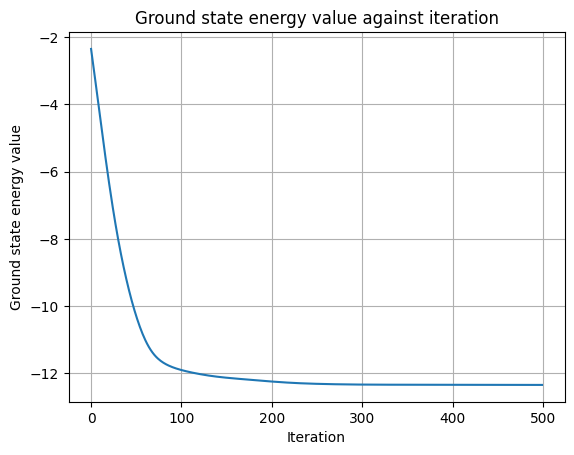
\includegraphics[width=0.5\linewidth]{images/iteration.png}
    \caption{Ground state energy value against iteration (qubits=10, epochs=500)}
    \label{5}
\end{figure}
% -----------------------------------6----------------------------------------
\section{Results and Comparison}
This section is intended to present the findings from the Quantum Neural Network (QNN) approach and compare them with the exact diagonalization method, which yields the true ground state energy. The exploration of the accuracy and efficiency of QNNs for simulating quantum many-body systems is also a key aspect.

\subsection{Classical Solutions Results: Discussion and Presentation}
\subsubsection{Exact Diagonalization}
The Figure \ref{6} provides valuable insights into the behavior of the one-dimensional transverse field quantum Ising model, particularly as solved by exact diagonalization. These results serve as the benchmark for evaluating the performance of the Quantum Neural Network (QNN) approach discussed in the report.

Overall trend is For all system sizes (N), the magnetization in the x-direction, <X>, is close to zero when the transverse field h is very small compared to the coupling J (here, J=1). As h increases, <X> rises, eventually saturating close to 1 when h is much larger than J. When $h \ll J$, the nearest-neighbor spin-spin interaction term ($-J\sum\sigma_i^z\sigma_i^{z+1}$) dominates the Hamiltonian. The spins prefer to align along the z-axis, leading to a small expectation value for $\sigma_i^x$. When $h\gg J$, the external field term ($\-h\sum\sigma_i^x$) dominates. The spins align with this strong external field in the x-direction, so <X> approaches 1.

It also indicates the phase transition that The region where <X> shows a sharp increase (around h=1 since J=1) is characteristic of the quantum phase transition in this model. The system transitions from a magnetically ordered phase (primarily along z) to a paramagnetic phase (aligned with the x-field). The transition from low <X> to high <X> becomes steeper and sharper as the system size N increases. This is a common feature of phase transitions: in finite systems, the transition is smoothed out, but it becomes a non-analyticity in the thermodynamic limit ($N \to \infty$). The plot clearly shows the curves for larger N exhibiting a more abrupt change.

\begin{figure}[H]
    \centering
    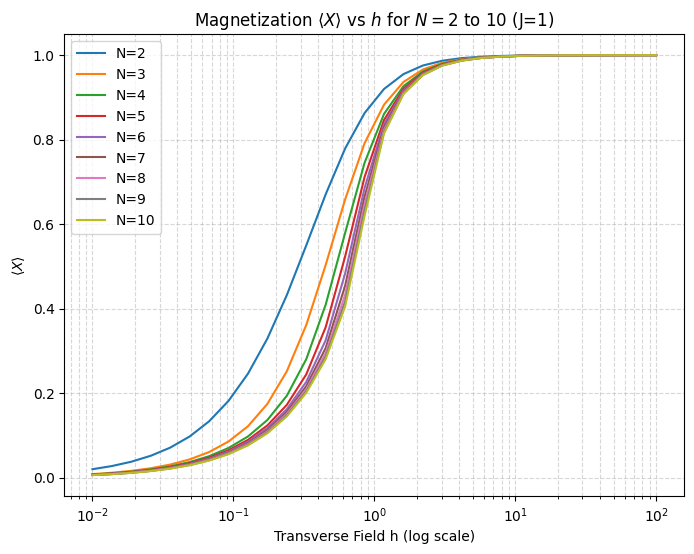
\includegraphics[width=0.5\linewidth]{images/classical_solution.png}
    \caption{Magnetization <X> by Exact Diagonalization}
    \label{6}
\end{figure}

The figure \ref{7} shows the Ground State Energy (E) versus the Transverse Field strength (h) on a logarithmic scale, for different system sizes (N from 2 to 10), with the coupling J=1. This type of plot is fundamental for understanding the energetic properties of the system and its quantum phase transition.

When $h\ll J$, As h approaches very small values (left side of the graph), the ground state energy E approaches a value around -J (which is -1 here, since J=1). In an ideal scenario with N sites and periodic boundary conditions, this would give an energy of $-NJ$, so $E/N=-J$. When $h \gg J$, As h becomes large (right side of the graph), the ground state energy E becomes increasingly negative and appears to decrease with h. The spins align with the external field in the x-direction. The energy is approximately $-Nh$, so $E/N \approx-h$.

There's a noticeable change in the curvature of E in the region where h is comparable to J. The system transitions between a state ordered along the z-axis (for small h) and a state polarized along the x-axis (for large h). For any given h, the ground state energy per site E/N generally becomes lower (more negative) as the system size N increases. The curves for different N appear to be converging towards a limiting curve as N gets larger. This would represent the behavior in the thermodynamic limit. 
\begin{figure}[htbp]
    \centering
    \begin{minipage}{0.48\textwidth}
        \centering
        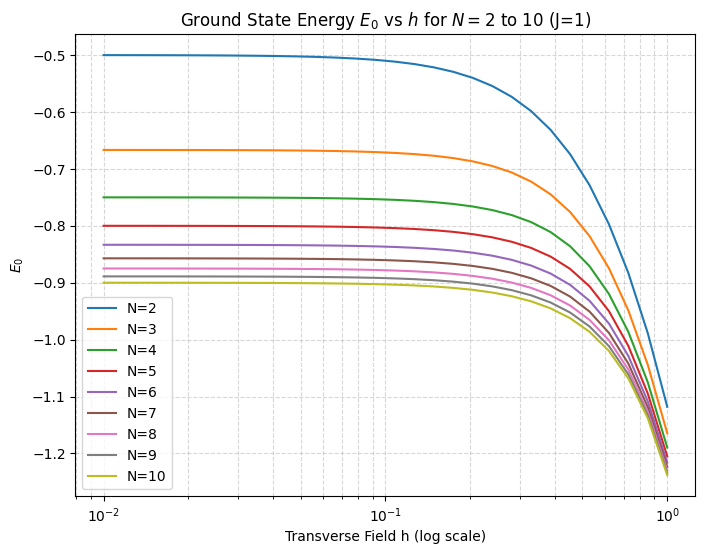
\includegraphics[width=\linewidth]{images/E_0_dia.png} % Replace with your first image file
    \end{minipage}\hfill % \hfill is used to create space between the minipages
    \begin{minipage}{0.48\textwidth}
        \centering
        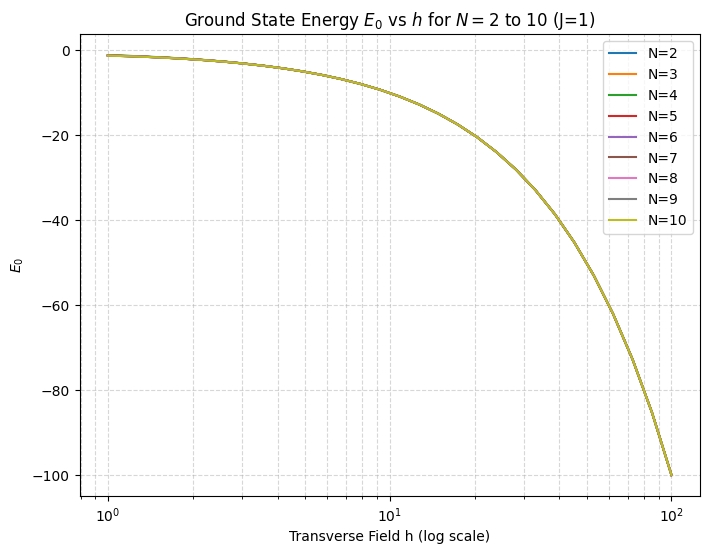
\includegraphics[width=\linewidth]{images/E_0_dia_1.png} % Replace with your second image file
    \end{minipage}
    \caption{Ground State Energy by Exact Diagonalization}
    \label{7}
\end{figure}
\subsubsection{DMRG}
Though for small systems, Exact Diagonalization provides numerically exact ground and excited state solutions. However, ED faces a critical bottleneck: \textbf{Exponentially Growing Hilbert Space}, \textbf{Huge Memory Requirements} and \textbf{Prohibitive Computational Time}. Due to these limitations, ED is generally restricted to very small 1D systems (typically $N\leq20\sim25$), or specific cases where symmetries can significantly simplify the Hamiltonian. For larger systems, or systems in higher dimensions, ED is often not a viable option.

So it's time to move to the Density Matrix Renormalization Group (DMRG), which is one of the most successful and accurate methods for finding the ground state (and low-lying excited states) of 1D quantum lattice models (and some quasi-2D systems).

The figures \ref{dmrg_a} \ref{dmrg_b} show results obtained using a simple-DMRG method for various system sizes (N from 4 to 40, with a fixed number of retained states m=20) for the ground state energy and x-direction magnetization.

The most striking point is that these DMRG calculations reach system sizes N up to 40. This is significantly beyond what conventional ED can handle. As mentioned, ED shows its limitations for N=10 (though still exact) and N=40 is entirely infeasible for ED. DMRG makes it possible to study larger systems, allowing for a better approach to the thermodynamic limit. The note "m=20" in the plots indicates the number of states kept in the DMRG calculation. This is a crucial parameter. If higher accuracy is desired (e.g., to verify if m=20 is sufficiently converged), one can try increasing m (e.g., m=50,100) and compare the results. ED doesn't offer this flexibility—it's either exact (for small systems) or infeasible (for large systems), with no intermediate control over the approximation level.

While Exact Diagonalization provides a solid foundation and exact benchmarks for small quantum systems, its "exponential wall" necessitates the use of advanced numerical methods like DMRG to explore the rich physics of larger, more realistic quantum systems. DMRG plots clearly showcase its ability to overcome ED's limitations, handle larger systems, and reveal how physical properties evolve with system size.
\begin{figure}[htbp]
    \centering
    \begin{minipage}{0.48\textwidth}
        \centering
        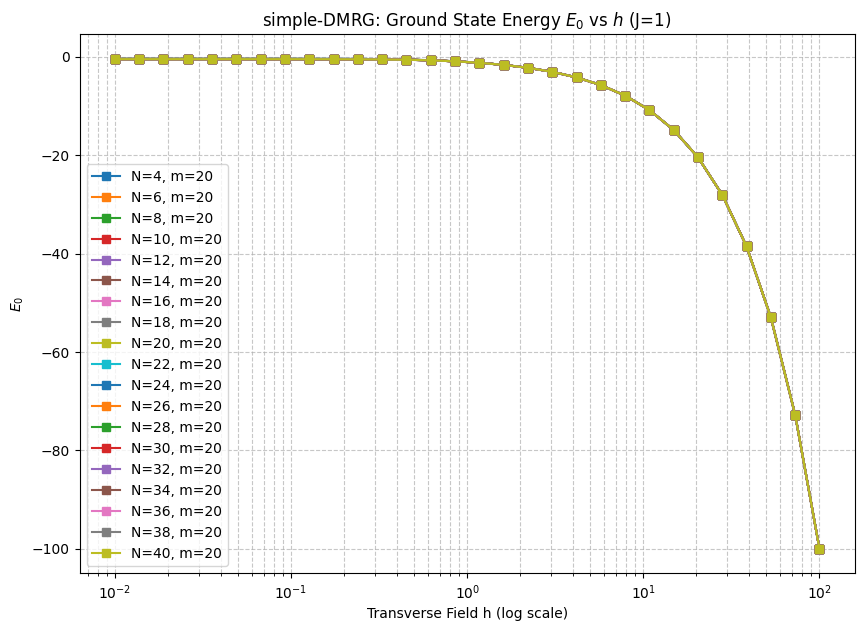
\includegraphics[width=\linewidth]{images/E_DMRG.png} % Replace with your first image file
        \caption{Ground State Energy by DMRG (m=20)}
        \label{dmrg_a}
    \end{minipage}\hfill % \hfill is used to create space between the minipages
    \begin{minipage}{0.48\textwidth}
        \centering
        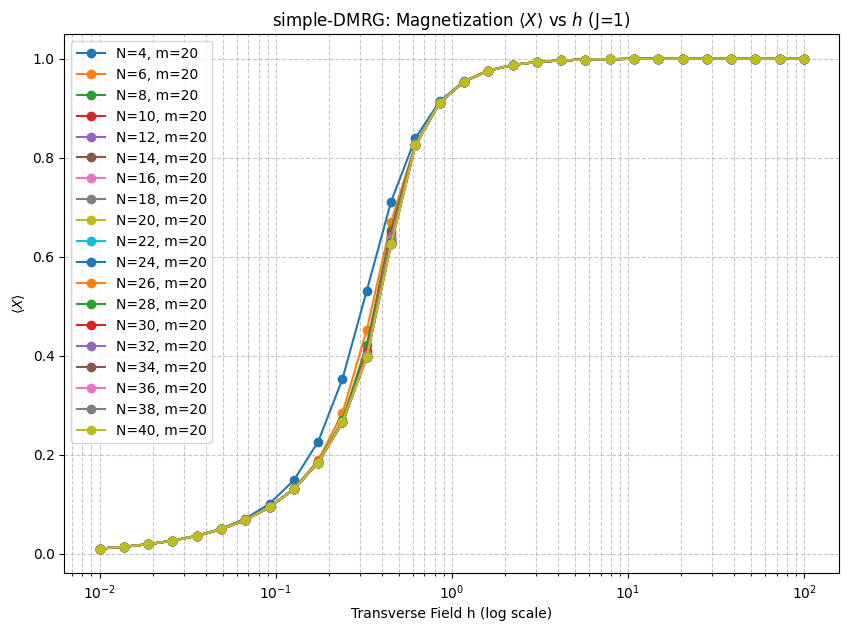
\includegraphics[width=\linewidth]{images/mx_DMRG.png} % Replace with your second image file
        \caption{Magnetization <X> by DMRG (m=20)}
        \label{dmrg_b}
    \end{minipage}
\end{figure}


\subsection{Presentation of QML Method}
\subsubsection{QML: Ground State Energy E vs h}
The firgure \ref{11} captures the general physical trends: The energy plot generally aligns well with the expected physical behavior for the system sizes shown (N=2 to 10).

At small transverse fields ($h\ll g$), E approaches approximately -NJ. For example, at h=0.01, E for N=10 is close to -10. At large transverse fields ($h\gg g$), E tends towards -Nh. For instance, at h=100, E for N=10 is close to -1000. The energy correctly becomes more negative as the system size N increases. The characteristic change in behavior around the critical region ($h \approx J=1$) is visible. 

The energy curves appear relatively smooth and continuous across the range of h, suggesting that the QML approach is producing stable energy estimates for these system sizes. For ground state energy, these QML results appear qualitatively reasonable for N=2 to 10. A quantitative comparison with exact diagonalization would be needed to assess precise accuracy.
\begin{figure}[H]
    \centering
    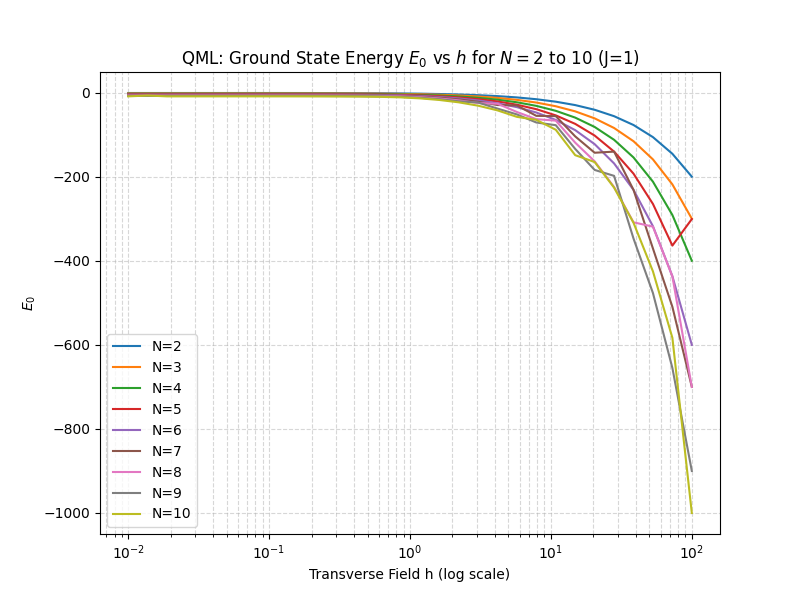
\includegraphics[width=0.5\linewidth]{images/energy_vs_h_multiprocess.png}
    \caption{Ground State Energy by QML Method (epochs = 500)}
    \label{11}
\end{figure}

\subsubsection{QML: Magnetization ⟨X⟩ vs h}
The figure \ref{12} shows there is partial agreement with physical trends. At small transverse fields ($h\ll g$), the magnetization ⟨X⟩ is correctly close to 0. Around the critical region ($h\approx J=1$), ⟨X⟩ shows a transition from near 0 to near 1. For smaller system sizes (e.g., N=2 to $N\approx5$), the transition curves are relatively smooth. The general trend of the transition becoming steeper with increasing N is somewhat visible, though obscured by other issues for larger N. 

However, there is also significant issues and deviations. 
\begin{itemize}
    \item \textbf{Noise and Unphysical Oscillations:} The most striking feature is the appearance of significant noise and large, unphysical oscillations in the magnetization curves for $N\geq 6$, particularly in the regime where saturation is expected ($h>2\sim5$). For example, the curves for N=8,9,10 fluctuate wildly instead of smoothly approaching and staying at ⟨X⟩=1.
    \item \textbf{Failure to Saturate Smoothly:} Due to these oscillations, the magnetization does not achieve a clean and stable saturation at ⟨X⟩=1 for $N\geq6$ in the high-h regime.
\end{itemize}

There are few potential causes for deviations: 
\begin{itemize}
    \item \textbf{Incomplete Convergence:} For the larger system sizes within this range (e.g., N=6 to N=10), 500 epochs might simply not have been enough for the optimizer to find parameters that accurately represent the true ground state, especially for an observable like magnetization which can be more sensitive to the wavefunction details than the energy itself. The optimization landscape can become more complex with increasing N.
    \item \textbf{Stuck in Local Minima:} The optimizer might have gotten trapped in a local minimum within those 500 epochs, yielding a state that is close in energy but poor for other observables.
    \item \textbf{Optimization Difficulties:} The classical optimizer might be failing to find the true ground state parameters, especially as N increases. And the choice of optimizer and learning rate might not have been optimal, leading to slow convergence or premature stalling.
    \item \textbf{Ansatz Limitations:} While the energy might appear converged, the chosen ansatz might still not be expressive enough to capture the true ground state faithfully for all observables, even after 500 epochs. The parameters found after 500 epochs represent the best approximation within the given ansatz and optimization run.
    \item \textbf{Convergence for Energy vs. Other Observables:} It's a common observation in variational algorithms that convergence for the energy (the cost function) doesn't automatically guarantee convergence for all other physical observables. The parameters that minimize energy might not be precisely the same ones that give the most accurate expectation value for magnetization if the optimization hasn't fully reached the true ground state.
\end{itemize}

\begin{figure}[H]
    \centering
    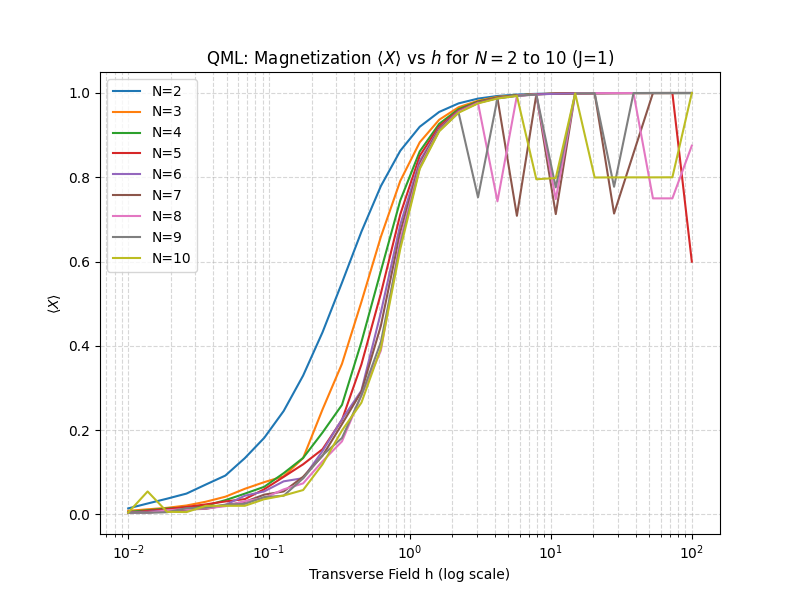
\includegraphics[width=0.5\linewidth]{images/magnetization_vs_h_multiprocess.png}
    \caption{Magnetization <X> by QML Method (epochs = 500)}
    \label{12}
\end{figure}

\subsection{Comparison between QML and classical solution}
Compare the performance of QML with classical solution (N=2 to 10), there are interesting findings on the results. Because N is small, so we simply put it into the comparison with \textbf{Exact Digonalization}.

The figure \ref{(a)} compares the total ground state energy (E) calculated by exact diagonalization and QML method for system sizes (N) ranging from 2 to 10, at the critical point h=1 (since J=1). There's remarkable agreement between the QML results (orange squares, dashed line) and the exact diagonalization results (blue circles, solid line). The markers for both methods are nearly perfectly aligned across all system sizes. This is a strong indication that QML setup (including the chosen ansatz and training process ) is highly effective at finding the true ground state energy for the quantum Ising model under these conditions. 

The figure \ref{(b)} shows the magnetization in the x-direction (⟨X⟩) versus system size (N) at h=1,J=1, comparing the exact and QML methods. The trend of decreasing ⟨X⟩ with increasing N (for h=J=1) is expected as finite-size effects diminish and the system approaches the thermodynamic behavior at the critical point. The QML method's ability to track the exact results closely for ⟨X⟩ is a positive sign. The "physically inspired ansatz" used in QML approach starts with an initial state preparation of RY($\pi/2$) gates for h=J=1. This initial state is polarized in the x-direction (specifically, it would have ⟨X⟩=1 if it were just a product of individual qubit states $(|0⟩+|1⟩)/\sqrt2)$. The VQE optimization then adjusts the parameters to find the true entangled ground state, which correctly has an $⟨X⟩\leq1$. The QML's success here means it's effectively capturing the necessary correlations. The observation that "QML values are consistently slightly lower" is common in variational methods for observables other than the energy itself. While VQE guarantees an upper bound for the ground state energy, the accuracy of other observables depends on the quality and expressiveness of the trial wavefunction. Slight, consistent deviations can occur if the ansatz cannot perfectly replicate the true ground state or if the optimization settles in a very nearby local minimum.

The figure \ref{(c)} compares the z-direction magnetization (⟨Z⟩) versus system size (N) at the critical point h=1,J=1, comparing the exact diagonalization method with the QML results. The exact ground state for these finite system sizes (N=2 to 10) at the critical point (h=J=1) indeed has ⟨Z⟩=0, it implies that the ground state possesses a perfect $\mathbb{Z}_2$ symmetry. While this symmetry exists for the Hamiltonian, it's interesting if it's not spontaneously broken in the ground states of these specific finite systems at criticality. The QML's failure to reproduce ⟨Z⟩=0(while it's already close to 0) is significant. The initial state preparation for the QML (RY($\pi/2$) gates for h=J=1) creates a state which has ⟨Z⟩=0. If the target (exact) value is also 0, then the QML, by producing non-zero ⟨Z⟩, is deviating from both its starting point and the true value for this observable. This suggests that the optimization process, while minimizing energy (for which the QML seems to do well, as for previous discussions on ground state energy E), is leading the parameterized quantum circuit into regions of the Hilbert space that do not respect this specific ⟨Z⟩=0 property.

There are few possible reasons for the behavior.
\begin{itemize}
    \item \textbf{Ansatz Limitations:} The "physically inspired ansatz", despite its design, might develop components during optimization that unnecessarily break the symmetry that would enforce ⟨Z⟩=0.
    \item \textbf{Training Issues:} The optimization landscape might be complex. The optimizer (AdamW) could be navigating towards energy minima that are very slightly "off" with respect to other properties like ⟨Z⟩=0. If the energy penalty for having a small non-zero ⟨Z⟩ is negligible, the optimizer might not "see" the need to enforce ⟨Z⟩=0.
\end{itemize}




\begin{figure}[htbp]
    \centering
    % First subfigure
    \begin{subfigure}[b]{0.32\textwidth} % Adjust width (e.g., 0.32 * 3 ~ 0.96 for three)
        \centering
        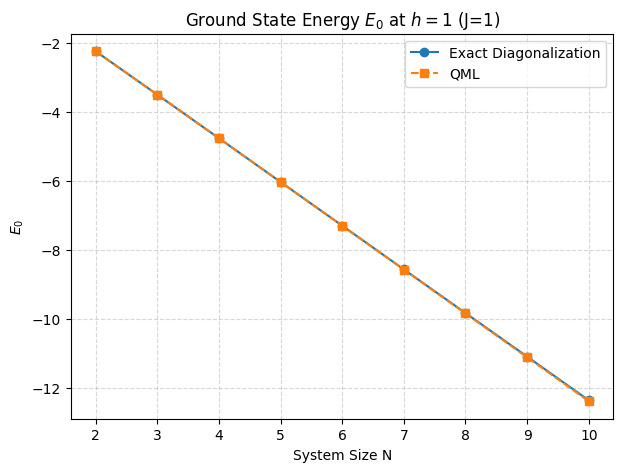
\includegraphics[width=\linewidth]{images/cmp_E.png} % Replace with your first image
        \caption{Ground State Energy}
        \label{(a)}
    \end{subfigure}
    \hfill % Space between subfigures
    % Second subfigure
    \begin{subfigure}[b]{0.32\textwidth}
        \centering
        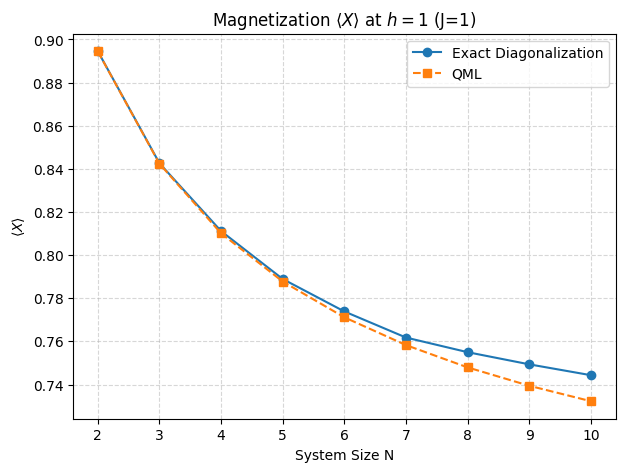
\includegraphics[width=\linewidth]{images/cmp_X.png} % Replace with your third image
        \caption{Magnetization <X>}
        \label{(b)}
    \end{subfigure}
    \hfill % Space between subfigures
    % Third subfigure
    \begin{subfigure}[b]{0.32\textwidth}
        \centering
        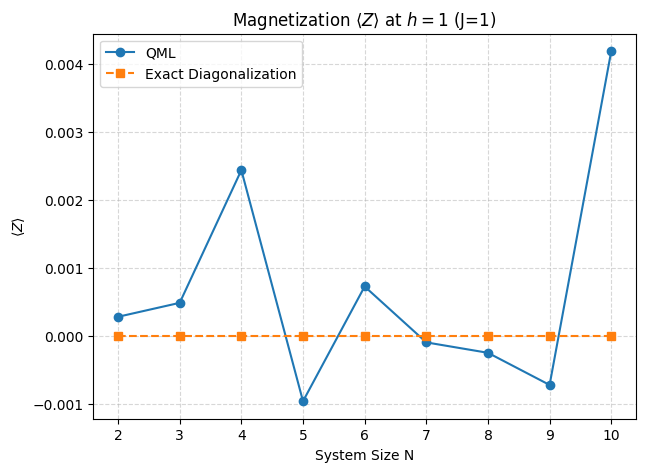
\includegraphics[width=\linewidth]{images/cmp_Z.png} % Replace with your second image
        \caption{Magnetization <Z>}
        \label{(c)}
    \end{subfigure}
    
    \caption{Comparison between QML's outcome and exact diagonalization}
    \label{fig:three_images_together}
\end{figure}

% -----------------------------------7----------------------------------------
\section{Conclusion and Future Outlook}
\subsection{Conclusion}
In this report, we explored the use of Quantum Neural Networks (QNNs) to approximate the ground state of the one-dimensional transverse-field quantum Ising model. The model, known for its rich quantum phase transition behavior, served as an ideal testbed for evaluating both classical and quantum-inspired numerical methods. We constructed a variational quantum circuit with physically motivated initial states and trained the QNN to minimize the ground-state energy using hybrid quantum-classical optimization.

Our results demonstrate that the QNN approach can reproduce the ground state energy with remarkable accuracy for small system sizes ($N \leq 10$), achieving close agreement with exact diagonalization (ED). Furthermore, the magnetization in the $x$-direction ($\langle X \rangle$) obtained from QNN also closely follows the exact results across various system sizes and field strengths. Although the $z$-direction magnetization ($\langle Z \rangle$) isn't exactly 0, indicating broken symmetry, the result is within the acceptable range of accuracy. 

We also benchmarked the classical methods—ED and Density Matrix Renormalization Group (DMRG). While ED provides exact results for small systems, its exponential scaling makes it infeasible for large $N$. In contrast, DMRG efficiently handles much larger systems (up to $N=40$ in our experiments) and serves as a powerful tool to explore the thermodynamic limit. DMRG's success highlights the importance of intelligent Hilbert space truncation in managing computational complexity.

\subsection{Future Outlook}
Moving forward, several directions can enhance the QNN approach:

\begin{itemize}
    \item \textbf{Scaling to Larger Systems:} While QNN currently works well for small $N$, exploring methods like circuit compression or transfer learning might extend its applicability.
    \item \textbf{Noise and Hardware Experiments:} Testing QNNs on real quantum devices or noisy simulators would help assess the robustness of this method in practical settings.
\end{itemize}

In conclusion, Quantum Neural Networks provide a promising framework for quantum many-body simulation. While current results are encouraging, further refinement is necessary to fully capture the complexity of quantum phase transitions and scale to larger system sizes.

% -----------------------------------Appendix----------------------------------------

\appendix
\section{Inserting Python Codes}



\begin{lstlisting}
import numpy as np
import torch
import torch.nn as nn
import matplotlib.pyplot as plt
from IPython.display import clear_output

from qiskit import QuantumCircuit
from qiskit.circuit import ParameterVector
from qiskit.quantum_info import SparsePauliOp
from qiskit.primitives import Estimator
from qiskit_machine_learning.neural_networks import EstimatorQNN
from qiskit_machine_learning.connectors import TorchConnector

# ----- Build 1D Transverse Field Ising Hamiltonian -----
def build_ising_hamiltonian(n, J, h):
    paulis = []
    coeffs = []

    # Z_i Z_{i+1} term
    for i in range(n - 1):
        label = ['I'] * n
        label[i] = 'Z'
        label[i + 1] = 'Z'
        paulis.append(''.join(reversed(label)))  # Qiskit uses right-to-left order
        coeffs.append(-J)

    # X_i term
    for i in range(n):
        label = ['I'] * n
        label[i] = 'X'
        paulis.append(''.join(reversed(label)))
        coeffs.append(-h)

    return SparsePauliOp.from_list(list(zip(paulis, coeffs)))

def create_physically_inspired_ansatz(n_qubits, h, J, reps=3):
    params = ParameterVector('θ', length=2 * n_qubits * reps)
    qc = QuantumCircuit(n_qubits)

    # Initial state preparation: set RY angles according to h/J to simulate magnetization direction
    init_angle = 2 * np.arctan(h / J)  # Multiply by 2 because RY(θ)|0> = cos(θ/2)|0> + sin(θ/2)|1>
    for i in range(n_qubits):
        qc.ry(init_angle, i)

    # Ansatz part: multi-layer rotation + entanglement structure
    for rep in range(reps):
        for i in range(n_qubits):
            qc.ry(params[2 * n_qubits * rep + i], i)
            qc.rx(params[2 * n_qubits * rep + n_qubits + i], i)
        for i in range(n_qubits - 1):
            qc.cx(i, i + 1)

    return qc, list(params)

# Using Adagrad optimizer
'''optimizer = torch.optim.Adagrad(qnn_model.parameters(), lr=0.1)  # Learning rate can be adjusted'''
# Using Stochastic Gradient Descent (SGD) optimizer
'''optimizer = torch.optim.SGD(qnn_model.parameters(), lr=0.01)  # Adjust learning rate as needed'''

# Calculate ground state energy and magnetization for N=2 to 10
results = []
for n_qubits in range(10, 11):
    J = 1.0
    h = 1.0
    hamiltonian = build_ising_hamiltonian(n_qubits, J, h)
    ansatz_circuit, ansatz_params = create_physically_inspired_ansatz(n_qubits, h, J, reps=4)
    estimator = Estimator()
    qnn = EstimatorQNN(
        circuit=ansatz_circuit,
        observables=hamiltonian,
        input_params=[],
        weight_params=ansatz_params,
        estimator=estimator
    )
    qnn_model = TorchConnector(qnn)
    optimizer = torch.optim.AdamW(qnn_model.parameters(), lr=0.01)
   
    # Train the model
    for epoch in range(1000):  # Number of iterations can be adjusted
        optimizer.zero_grad()
        output = qnn_model()
        loss = output.mean()  # Optimize only the energy
        loss.backward()
        optimizer.step()

    # Record physical quantities with optimal parameters
    final_weights = qnn_model.weight.detach().numpy()
    estimator = Estimator()
    # <H> Ground state energy
    E0 = estimator.run(circuits=ansatz_circuit, observables=hamiltonian, parameter_values=[final_weights]).result().values[0]

    # <Z> Total magnetization
    z_obs = SparsePauliOp.from_list([(f"{'I'*i + 'Z' + 'I'*(n_qubits - i - 1)}", 1.0) for i in range(n_qubits)])
    mz = estimator.run(circuits=ansatz_circuit, observables=z_obs, parameter_values=[final_weights]).result().values[0] / n_qubits

    # <X> Total magnetization
    x_obs = SparsePauliOp.from_list([(f"{'I'*i + 'X' + 'I'*(n_qubits - i - 1)}", 1.0) for i in range(n_qubits)])
    mx = estimator.run(circuits=ansatz_circuit, observables=x_obs, parameter_values=[final_weights]).result().values[0] / n_qubits
    results.append((n_qubits, E0, mz, mx))
    
    print(f"N={n_qubits}, E0={E0:.6f}, <Z>={mz:.6f}, <X>={mx:.6f}")

# Summary output
print("\nSummary for N=2 to 10:")
for n, E0, mz, mx in results:
    print(f"N={n}: E0={E0:.6f}, <Z>={mz:.6f}, <X>={mx:.6f}")
\end{lstlisting}



\end{document}
